\part{Electromagnetism}
\chapter{Fundamentals}
\section{Maxwell's equations}
As we studied in previous courses all the classical Electromagnetism is contained in some fundamental equations. Those are the Maxwell's equations and the Lorentz force. Maxwell's equations can be either in integral form or differential form. Let's start from the integral form in a vacuum:
\begin{equation} \label{e:int_Maxwell_eq}
  \begin{split}
    &\oint_{\Sigma} \vec{E} \cdot \dd{\vec{\Sigma}} = \dfrac{Q_{enc}}{\epsz}\\[8pt]
    &\oint_{\Sigma} \vec{B} \cdot \dd{\vec{\Sigma}} = 0\\[8pt]
    &\oint_{\gamma} \vec{E} \cdot \dd{\vec{s}} = \dv{}{t}\int_{\Sigma} \vec{B} \cdot \dd{\vec{\Sigma}}\\[8pt]
    &\oint_{\gamma} \vec{B} \cdot \dd{\vec{s}} = \muz i_{enc} + \muz \epsz \dv{}{t}\int_{\Sigma} \vec{E} \cdot \dd{\vec{\Sigma}}
  \end{split}
\end{equation}
The differential (or local) form can be written using various calculus theorem such as stokes theorem or the divergence theorem:
\begin{equation} \label{e:diff_Maxwell_eq}
  \begin{split}
    &\div{\vec{E}} = \dfrac{\rho}{\epsz}\\[8pt]
    &\div{\vec{B}} = 0\\[8pt]
    &\curl{\vec{E}} = -\pdv{\vec{B}}{t}\\[8pt]
    &\curl{\vec{B}} = \muz \vec{J} + \muz \epsz \pdv{\vec{E}}{t}
  \end{split}
\end{equation}
If we want to write Maxwell's equation in materials we must slightly change our definitions. First we must identify new fields which we will call $\vec{D}$ field and $\vec{H}$ field.
Also, inside matter, we can distinguish two "types" of charges: the \textbf{free charges} and the \textbf{polarization charges}. This means that for the electric field:
\begin{equation}
  \begin{split}
    Q &\rightarrow Q_f + Q_{pol}\\[8pt]
    \rho &\rightarrow \rho_f + \rho_{pol}
  \end{split}
\end{equation}
For the magnetic field we must distinguish two currents: the \textbf{free current} and the \textbf{magnetic current} (given by the bounded charges and the polarization charges). From this we get that:
\begin{equation}
  \begin{split}
    i &\rightarrow i_f + i_b + i_p\\[8pt]
    \vec{J} &\rightarrow \vec{J}_f + \vec{J}_b + \vec{J}_p
  \end{split}
\end{equation}
Finally we can write Maxwell's equations in matter:
\begin{equation} \label{e:Maxwell_matter}
  \begin{split}
    &\div{\vec{D}} = \rho_f\\[8pt]
    &\div{\vec{B}} = 0\\[8pt]
    &\curl{\vec{E}} = -\pdv{\vec{B}}{t}\\[8pt]
    &\curl{\vec{H}} = \vec{J}_f + \pdv{\vec{D}}{t}
  \end{split}
\end{equation}
Those equations + the Lorentz force can describe all classical Electromagnetism. The expression of the Lorentz force is:
\begin{equation}
  \vec{F} = q (\vec{E} + \vec{v} \cross \vec{B})
\end{equation}
In the stationary case \maxwellref\;become:
\begin{equation} \label{e:stationary_Maxwell_eq}
  \begin{split}
    &\div{\vec{E}} = \dfrac{\rho}{\epsz}\\[8pt]
    &\div{\vec{B}} = 0\\[8pt]
    &\curl{\vec{E}} = 0\\[8pt]
    &\curl{\vec{B}} = \muz \vec{J}
  \end{split}
\end{equation}
The third equation tells us that $\vec{E}$ is an irrotational field in the stationary case. Also, contrary to the general equations, in the stationary case the electric field and the magnetic field are independent.\\
Since the electrostatic field is irrotational we can write it as the gradient of some scalar field since it is always true that:
\begin{equation}
  \curl{(\grad{f})} = 0 \quad \forall f(\vec{r})
\end{equation}
Thus we define the \textbf{electrostatic potential} $\potE$ such that:
\begin{equation}
  \vec{E} = -\grad{\potE}
\end{equation}
Let's now calculate the work of the electromagnetic field in the stationary case over a moving particle with charge $q$. Using the Lorentz force we get:
\begin{equation}
  W_{AB} = \int_{A}^{B} q (\vec{E} + \vec{v} \cross \vec{B}) \cdot \dd{\vec{s}} = \int_{A}^{B} q \vec{E} \cdot \dd{\vec{s}} + \int_{A}^{B} \vec{v} \cross \vec{B} \cdot \dd{\vec{s}}
\end{equation}
Since $\vec{v} \cross \vec{B} \parallel \vec{s}$ the second integral is zero, thus we get:
\begin{equation}
  \begin{split}
    W_{12} &= \int_{A}^{B} q \vec{E} \cdot \dd{\vec{s}} =\\[8pt]
    &= -q \int_{A}^{B} \grad{\potE} \cdot \dd{\vec{s}} =\\[8pt]
    &= -q \int_{A}^{B} \dd{\potE} = q\potE(A) - q\potE(B)
  \end{split}
\end{equation}
So the work of the electrostatic field is just given by the difference between the values of the potential of the two points. Keep in mind that only the difference $\potE(A) - \potE(B)$ has physical meaning. The potential itself can be changed of a constant and the work would be the same. Usually we want to set the reference point for the potential at infinity and so the work necessary to bring a charge from point $A$ to infinity is:
\begin{equation}
  W_{A\rightarrow +\infty} = q\potE(A) - \underbrace{q\potE(+\infty)}_{=\;0} = q\potE(A)
\end{equation}
Now let's imagine a charge fixed at a point $\vec{r}'$ that generates an electrostatic field in space.
\begin{figure}[H]
  \centering
  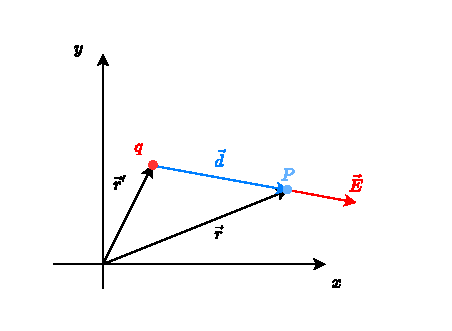
\includegraphics[width=0.7\linewidth]{res/svg/point_charge.drawio}
  \caption{Point charge in space}
\end{figure}
We want to calculate the potential and the electric field at a point $\vec{r}$. The potential only depends on the distance between the points which we will denote with the vector $\vec{d}$. Actually the potential only depends on the modulus of the distance which is $d = \norm{\vec{r}-\vec{r}'}$. Instead, the electric field is given by Coulomb's law:
\begin{equation}
  \vec{E}(\vec{r}) = \dfrac{1}{4 \pi \epsz}\dfrac{Q}{\norm{\vec{r}-\vec{r}'}^3}\brackets{\vec{r}-\vec{r}'}
\end{equation}
We could define a radial versor $\hat{u}_r \defineeq \dfrac{\vec{r}-\vec{r}'}{\norm{\vec{r}-\vec{r}'}}$, but this would be essentially useless, instead with the given notation we do not need to account for extra stuff during calculations.\\
Now, instead of a single point charge, we imagine putting $n$ charges in space and we still want to evaluate the electric field at $\vec{r}$. To do this we simply add (vectorially) all the contributions of the charges:
\begin{equation}
  \vec{E}(\vec{r}) = \bigsum_i\dfrac{1}{4 \pi \epsz}\dfrac{Q_i}{\norm{\vec{r}-\vec{r}_i'}^3}\brackets{\vec{r}-\vec{r}_i'}
\end{equation}
Same goes for the potential:
\begin{equation}
  \potE(\vec{r}) = \bigsum_i\dfrac{1}{4 \pi \epsz}\dfrac{Q_i}{\norm{\vec{r}-\vec{r}_i'}}
\end{equation}
If instead of a finite number of point charges we are dealing with a continuous distribution of charges we simply "switch" the discrete summation with an integral and integrate over all charges:
\begin{equation}
  \potE(\vec{r}) = \dfrac{1}{4 \pi \epsz}\int_Q \dfrac{\dd{q}}{\norm{\vec{r}-\vec{r}'}}
\end{equation}
The infinitesimal element $\dd{q}$ just represents the charge of an infinitesimal volume $\dd{\tau}$ and so, given the distribution's density we can say that $\dd{q} = \rho \dd{\tau} = \rho \dd{^3 \vec{r}}$, but we need to remind that we are now integrating over a volume. So the new formula becomes:
\begin{equation} \label{e:general_sol_poisson}
  \potE(\vec{r}) = \dfrac{1}{4 \pi \epsz}\int_{\tau} \dfrac{\rho (\vec{r}')}{\norm{\vec{r}-\vec{r}'}}\dd{^3 \vec{r}}
\end{equation}
There is another immediate property of the potential $\potE$. If we simply substitute $-\grad{\potE}$ in the first Maxwell equation we get:
\begin{equation}
  \div{\vec{E}} = \div{\brackets{-\grad{\potE}}} = -\lap{\potE} = \dfrac{\rho}{\epsz}
\end{equation}
The last equation can be simply rewritten as:
\begin{equation} \label{e:Poisson_eq}
  \boxed{\lap{\potE} = -\dfrac{\rho}{\epsz}}
\end{equation}
Which is called \textbf{Poisson's equation}. We can do a similar thing for the vector potential $\vec{A}$. We recall that this property is true:
\begin{equation}
  \curl{(\curl{\vec{C}})} = \grad{(\div{\vec{C}})} - \lap{\vec{C}}
\end{equation}
The laplacian operator, in this case, is inteded as applied to every component of $\vec{C}$. To apply this to the vector potential we simply substitute $\vec{B} = \curl{\vec{A}}$ in the fourth Maxwell equation (stationary case):
\begin{equation}
  \grad{(\div{\vec{A}})} - \lap{\vec{A}} = \muz \vec{J}
\end{equation}
And so finally we arrived to this set of equation:
\begin{equation} \label{e:pot_stat_eq}
  \begin{split}
    &\lap{\potE} = -\dfrac{\rho}{\epsz}\\[8pt]
    &\grad{(\div{\vec{A}})} - \lap{\vec{A}} = \muz \vec{J}
  \end{split}
\end{equation}
Which is a set of 4 equations (1 for $\potE$, 3 for $\vec{A}$) which are completely equivalent to \maxwellref\;in the stationary case, since we derived them from \maxwellref\;themselves.\\
Let's continue with the non-stationary case. The divergence of $\vec{B}$ will still be:
\begin{equation}
  \div{\vec{B}} = 0
\end{equation}
Thus, we can still define a vector potential in the same way we did for the stationary case:
\begin{equation}
  \vec{B} = \curl{\vec{A}}
\end{equation}
But looking at the third \maxwellref\;we get:
\begin{equation}
  \curl{\vec{E}} = -\pdv{}{t}\curl{\vec{A}}
\end{equation}
And so the field $\vec{E}$ itself is not irrotational anymore. Instead, if we bring all the terms to one side we have:
\begin{equation}
  \curl{\brackets{\vec{E} + \pdv{\vec{A}}{t}}} = 0
\end{equation}
And so $\vec{E} + \pdv{\vec{A}}{t}$ is irrotational. We can thus define a new scalar potential with the form:
\begin{equation}
  -\grad{\potE} = \vec{E} + \pdv{\vec{A}}{t}
\end{equation}
And so the electric field $\vec{E}$ will now be:
\begin{equation}
  \vec{E} =  -\grad{\potE} -\pdv{\vec{A}}{t}
\end{equation}
So the first Maxwell equation becomes:
\begin{equation}
  \begin{split}
    \div{\vec{E}} &= \div{\brackets{-\grad{\potE} -\pdv{\vec{A}}{t}}} = \\[8pt]
    &= \boxed{-\lap{\potE} -\pdv{}{t}\div{\vec{A}} = \dfrac{\rho}{\epsz}}
  \end{split}
\end{equation}
The fourth Maxwell equation will now simply be:
\begin{equation}
  \boxed{\grad{\brackets{\div{\vec{A}}}} - \lap{\vec{A}} = \muz \vec{J} + \muz \epsz \pdv{}{t}\brackets{-\grad{\potE} - \pdv{\vec{A}}{t}}}
\end{equation}
\section{Gauge transformations}
In this section we will introduce a type of transformation which will help us to achieve a more compact and elegant way to write \maxwellref.
\begin{definition}{Gauge transformations}
  Gauge transformations are transformations of the potentials that leave the fields unchanged
\end{definition}
\noindent In the static case a simple gauge transformation for the electric field can be:
\begin{equation}
  \begin{split}
    &\potE \longrightarrow \potE' = \potE + c\\[8pt]
    \implies &-\grad{\potE'} = -\grad{\brackets{\potE + c}} = -\grad{\potE} - \cancel{\grad{c}} = -\grad{\potE} = \vec{E}\\[8pt]
    &-\grad{\potE'} = \vec{E}
  \end{split}
\end{equation}
Obviously the field $\vec{E}$ remains the same since the gradient of a function is invariant under translation of that function. Similarly, we can do a simple transformation for the potential vector:
\begin{equation}
  \begin{split}
    &\vec{A} \longrightarrow \vec{A}' = \vec{A} + \grad{\xi}\\[8pt]
    \implies &\curl{\vec{A}'} = \curl{\brackets{\vec{A} + \grad{\xi}}} = \curl{\vec{A}} + \cancel{\curl{\grad{\xi}}} = \curl{\vec{A}} = \vec{B}\\[8pt]
    &\curl{\vec{A}'} = \vec{B}
  \end{split}
\end{equation}
Where the function $\xi (\vec{x})$ is called \textbf{Gauge function} and is a function of only the coordinates. As we anticipated we can exploit those transformations to simplify the equations we previously got. In particular if we make a gauge transformation such that:
\begin{equation}
  \div{\vec{A}'} = 0
\end{equation}
Then the second equation in \eqref{e:pot_stat_eq} becomes:
\begin{equation}
  \begin{split}
    \grad{(\cancel{\div{\vec{A}'}})} - \lap{\vec{A}'} &= \muz \vec{J}\\[8pt]
    \lap{\vec{A}'} &= -\muz \vec{J}
  \end{split}
\end{equation}
This transformation is thus defined as:
\begin{definition}{Coulomb gauge}
  The Coulomb gauge is a transformation such that:
  \begin{equation}
    \div{\vec{A}'} = 0
  \end{equation}
\end{definition}
\noindent In order to be able to perform this transformation we need to choose a proper functional form of $\xi$. By using the definition we have:
\begin{equation}
  \begin{split}
    &\div{\brackets{\vec{A}+\grad{\xi}}} \overset{!}{=} 0 \\[8pt]
    &\div{\vec{A}} + \lap{\xi} = 0 \\[8pt]
    &\boxed{\lap{\xi} = -\div{\vec{A}}}
  \end{split}
\end{equation}
So this is the condition that $\xi$ must obey in order to generate the Coulomb gauge. Obviously we can make another transformation in the Coulomb gauge that remanis in the Coulomb gauge. Repeating the steps we did for the general condition we get:
\begin{equation}
  \begin{split}
    &\div{\brackets{\vec{A}'+\grad{\xi'}}} \overset{!}{=} 0 \\[8pt]
    &\cancel{\div{\vec{A}'}} + \lap{\xi'} = 0 \\[8pt]
    &\lap{\xi'} = 0
  \end{split}
\end{equation}
This means that the function must be harmonic.\\
In conclusion, for the stationary case we can sum up the equations of the potential in the Coulomb gauge in a single form:
\begin{equation}
  \lap{\psi} = -s
\end{equation}
Where:
\begin{itemize}
  \item $\psi$ is the potential, either $\potE$ or a component $A_i$
  \item $s$ is the source of the field, either $\rho/\epsz$ or $\muz J_i$
\end{itemize}
Now let's move on to the general case (non-stationary case). We can still start from the basic transformation for the vector potential, but in this case we get:
\begin{equation}
  \begin{split}
    \vec{E} &\overset{!}{=} -\grad{\potE'} - \pdv{\vec{A'}}{t} \\[8pt]
    -\grad{\potE} - \cancel{\pdv{\vec{A}}{t}} &= -\grad{\potE'} - \pdv{}{t}\brackets{\cancel{\vec{A}} + \grad{\xi}} \\[8pt]
    \grad{\potE} &= \grad{\potE'} + \pdv{}{t}\brackets{\grad{\xi}} \\[8pt]
    \potE' &= \potE - \pdv{\xi}{t}
  \end{split}
\end{equation}
So this is the second "basic transformation" in the general case. Keep in mind that we are looking for a way to further simplify these equations:
\begin{equation}
  \begin{split}
    &-\lap{\potE} -\pdv{}{t}\div{\vec{A}} = \dfrac{\rho}{\epsz} \\[8pt]
    &\grad{\brackets{\div{\vec{A}}+ \dfrac{1}{c^2}\pdv{\potE}{t}}} - \lap{\vec{A}} + \dfrac{1}{c^2} \pdv[2]{\vec{A}}{t} = \muz \vec{J}
  \end{split}
\end{equation}
We define a new transformation:
\begin{definition}{Lorentz gauge}
  The Lorentz gauge is a gauge transformation such that:
  \begin{equation} \label{e:Lorentz_gauge}
    \div{\vec{A}'}+ \dfrac{1}{c^2}\pdv{\potE'}{t} = 0
  \end{equation}
\end{definition}
If we succed in finding this transformation the second equations then become:
\begin{equation}
  \begin{split}
    &\lap{\potE'} - \dfrac{1}{c^2} \pdv[2]{\potE'}{t} = -\dfrac{\rho}{\epsz} \\[8pt]
    &\lap{\vec{A}'} - \dfrac{1}{c^2} \pdv[2]{\vec{A}'}{t} = -\muz \vec{J}
  \end{split}
\end{equation}
We can easily spot the simmetry of those equations. In particular, we now define a new operator:
\begin{definition}{D'Alembert operator}
  The D'Alembert operator is an operator constructed as follows:
  \begin{equation}
    \dalop \defineeq \lap - \dfrac{1}{c^2} \pdv[2]{}{t}
  \end{equation}
\end{definition}
And so the equations can be rewritten as:
\begin{equation}
  \begin{split}
    &\dalop \potE' = -\dfrac{\rho}{\epsz} \\[8pt]
    &\dalop \vec{A}' = -\muz \vec{J}
  \end{split}
\end{equation}
We still need to understand if this transformation is possible. Recall that the possible basic transformations in this case are:
\begin{equation}
  \begin{split}
    &\potE \longrightarrow \potE' = \potE - \pdv{\xi}{t}\\[8pt]
    &\vec{A} \longrightarrow \vec{A}' = \vec{A} + \grad{\xi}
  \end{split}
\end{equation}
And we want to achieve \eqref{e:Lorentz_gauge}. By substituting we get:
\begin{equation}
  \begin{split}
    &\div{\brackets{\vec{A} + \grad{\xi}}} + \dfrac{1}{c^2} \pdv{}{t}\brackets{\potE - \pdv{\xi}{t}} = 0 \\[8pt]
    &\div{\vec{A}} + \lap{\xi} + \dfrac{1}{c^2} \pdv{\potE}{t} - \dfrac{1}{c^2} \pdv[2]{\xi}{t} = 0 \\[8pt]
    &\lap{\xi} - \dfrac{1}{c^2} \pdv[2]{\xi}{t} = -\div{\vec{A}} - \dfrac{1}{c^2} \pdv{\potE}{t} \\[8pt]
    &\boxed{\dalop \xi = -\brackets{\div{\vec{A}} + \dfrac{1}{c^2} \pdv{\potE}{t}}}
  \end{split}
\end{equation}
As for the Coulomb gauge we can make a transformation in the Lorentz gauge and stay in the Lorentz gauge. Similarly to what we got before the condition for the new gauge function will be:
\begin{equation}
  \dalop \xi' = 0
\end{equation}
\section{Solutions to the potential equations}
Now that we have the equations for the potentials in a more compact way we can ask ourselves what the solutions to those equations are. We already know that the most general solution for $\potE$ \underline{in the static case} is:
\begin{equation}
  \potE(\vec{r}) = \dfrac{1}{4 \pi \epsz}\int_{\tau} \dfrac{\rho (\vec{r}')}{\norm{\vec{r}-\vec{r}'}}\dd{^3 \vec{r}}
\end{equation}
Not so surprisingly the solution for each component of $\vec{A}$ will be something very similar to this solution. In particular, it will be:
\begin{equation}
  A_i(\vec{r}) = \dfrac{\muz}{4 \pi }\int_{\tau} \dfrac{J_i}{\norm{\vec{r}-\vec{r}'}}\dd{^3 \vec{r}}
\end{equation}
And so we can write the solutions in the compact form:
\begin{equation} \label{e:pot_general_solutions}
  \begin{split}
    &\potE(\vec{r}) = \dfrac{1}{4 \pi \epsz}\int_{\tau} \dfrac{\rho (\vec{r}')}{\norm{\vec{r}-\vec{r}'}}\dd{^3 \vec{r}} \\[8pt]
    &\vec{A}(\vec{r}) = \dfrac{\muz}{4 \pi }\int_{\tau} \dfrac{\vec{J} (\vec{r}')}{\norm{\vec{r}-\vec{r}'}}\dd{^3 \vec{r}}
  \end{split}
\end{equation}
Actually the volume element in the second equation is just the volume of the cable where the current generating the field is passing thus it can be explicited as:
\begin{equation}
  \dd{\tau} = \Sigma \dd{l}
\end{equation}
\begin{figure}[H]
  \centering
  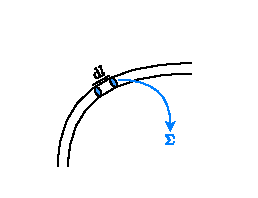
\includegraphics[width=0.5\linewidth]{res/svg/cable.drawio}
  \caption{Wire element}
\end{figure}
Since $J\Sigma = i$ if we "pass" the unit vector of $\vec{J}$ to the infinitesimal length element we obtain an integration of the current only over the circuit:
\begin{equation}
  \vec{A}(\vec{r}) = \dfrac{\muz}{4 \pi }\int_{\gamma} \dfrac{i \dd{\vec{l}}}{\norm{\vec{r}-\vec{r}'}}
\end{equation}
Now we want to prove that the general solution stated in \eqref{e:pot_general_solutions} is indeed a solution. We simply verify that $\vec{B} = \curl{\vec{A}}$:
\begin{equation}
  \begin{split}
    \curl{\vec{A}} &= \curl \dfrac{\muz}{4 \pi }\int_{\tau} \dfrac{\vec{J} (\vec{r}')}{\norm{\vec{r}-\vec{r}'}}\dd{^3 \vec{r}} \\[8pt]
    &=  \dfrac{\muz}{4 \pi }\int_{\tau} \curl{\brackets{\dfrac{\vec{J} (\vec{r}')}{\norm{\vec{r}-\vec{r}'}}}} \dd{^3 \vec{r}}
  \end{split}
\end{equation}
Now we need to exploit this identity:
\begin{equation}
  \curl{\brackets{\vec{f}g}} = g\curl{\vec{f}} + \grad{g} \cross \vec{f}
\end{equation}
In our equation this will result in:
\begin{equation}
  \begin{split}
    &\dfrac{\muz}{4 \pi }\int_{\tau} \curl{\brackets{\dfrac{\vec{J} (\vec{r}')}{\norm{\vec{r}-\vec{r}'}}}} \dd{^3 \vec{r}} = \\[8pt]
    &= \dfrac{\muz}{4 \pi }\int_{\tau}\left[ \cancel{\curl{\brackets{\vec{J}(\vec{r}')}}}\dfrac{1}{\norm{\vec{r}-\vec{r}'}}  + \grad{\brackets{\dfrac{1}{\norm{\vec{r}-\vec{r}'}}}} \cross \vec{J}(\vec{r}')\right]\dd{^3 \vec{r}}
  \end{split}
\end{equation}
The curl of $\vec{J}$ is zero since it does not depend on the coordinates $x,y,z$ of the gradient. For the gradient of the norm of the distance we just explicit the calculation. For the partial derivative with respect to $x$ we have:
\begin{equation}
  \begin{split}
    \pdv{}{x}\brackets{\dfrac{1}{\sqrt{(x-x')^2 + (y-y')^2 + (z-z')^2}}} = -\dfrac{\cancel{2}(x-x')}{\cancel{2}\left[(x-x')^2 + (y-y')^2 + (z-z')^2\right]^{3/2}}
  \end{split}
\end{equation}
The result will be essentially the same for the other components thus the integral now becomes:
\begin{equation}
  \dfrac{\muz}{4 \pi }\int_{\tau}-\brackets{\dfrac{\vec{r}-\vec{r}'}{\norm{\vec{r}-\vec{r}'}^3}} \cross \vec{J}(\vec{r}')\dd{^3 \vec{r}}
\end{equation}
If we switch the order of the cross product we must change sign, also we can apply the trick we explained before to integrate over the circuit, and so we end up with:
\begin{equation}
  \dfrac{\muz}{4 \pi }\int_{\gamma}\dfrac{i \dd{\vec{l}} \cross \brackets{\vec{r}-\vec{r}'}}{\norm{\vec{r}-\vec{r}'}^3}
\end{equation}
Now we want to find a general solution for the \underline{non-stationary} case of the potential equations. Our problem is solved if we find a general solution to this equation:
\begin{equation}
  \dalop \psi = -s
\end{equation}
Then we can easily adapt it to the different sources and potentials we can possibly have. Now imagine being far from the source, in this case the contirbution of $s$ goes to zero and we have:
\begin{equation}
  \dalop \psi = 0
\end{equation}
Which is just the D'Alembert equation. Suppose that we have a single spherical source in the origin and we want to calculate the potential $\psi (P)$ in a point $P$ very far from the source.
\begin{figure}[H]
  \centering
  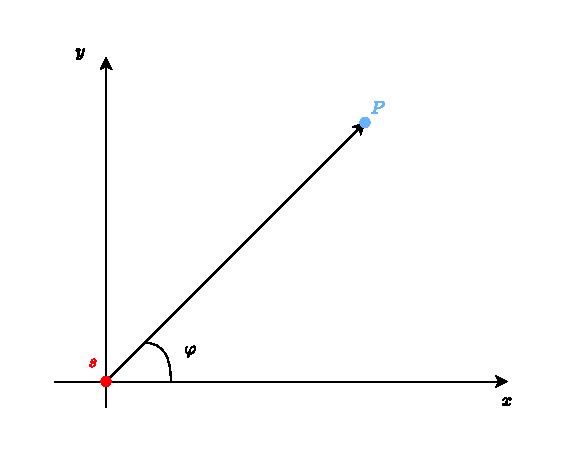
\includegraphics[width=0.7\linewidth]{res/svg/long_distance_potential.drawio}
  \caption{Long distance potential}
\end{figure}
Since we are considering a spherical simmetry we should use D'Alembert in spherical coordinates. We just need to change the laplacian which can be written as:
\begin{equation}
  \lap = \dfrac{1}{r^2} \pdv{}{r}\left(r^2 \pdv{}{r}\right) + \dfrac{1}{r^2 \sin{\theta}} \pdv{}{\theta}\left(\sin{\theta} \pdv{}{\theta}\right) + \dfrac{1}{r^2 \sin^2{\theta}} \pdv[2]{}{\varphi}
\end{equation}
Since in our case there is no dependence on $\theta$ or $\varphi$ the D'Alembert operator applied to $\psi$ results in:
\begin{equation} \label{e:dalop_far_source}
  \dalop \psi = \dfrac{1}{r^2} \pdv{}{r}\left(r^2 \pdv{\psi}{r}\right) - \dfrac{1}{c^2} \pdv[2]{\psi}{t} = 0
\end{equation}
Let's evaluate the first term:
\begin{equation}
  \dfrac{1}{r^2} \pdv{}{r}\left(r^2 \pdv{\psi}{r}\right) = \dfrac{1}{r^2} \left[2r \pdv{\psi}{r} + r^2 \pdv[2]{\psi}{r}\right] = \dfrac{2}{r} \pdv{\psi}{r} + \pdv[2]{\psi}{r}
\end{equation}
Which can also be seen as:
\begin{equation}
  \begin{split}
    &\dfrac{1}{r} \pdv{\psi}{r} + \dfrac{1}{r} \pdv{\psi}{r} + \pdv[2]{\psi}{r} = \dfrac{1}{r} \pdv{\psi}{r} + \dfrac{1}{r}\pdv{}{r}\brackets{r\pdv{\psi}{r}} = \\[8pt]
    &= \dfrac{1}{r} \pdv{}{r}\brackets{\psi + r\pdv{\psi}{r}} = \dfrac{1}{r}\pdv{}{r}\brackets{\pdv{\brackets{r\psi}}{r}} = \dfrac{1}{r}\pdv[2]{\brackets{r\psi}}{r}
  \end{split}
\end{equation}
And so \eqref{e:dalop_far_source} can be rewritten as:
\begin{equation}
  \pdv[2]{\brackets{r\psi}}{r} - \dfrac{1}{c^2} \pdv[2]{\brackets{r\psi}}{t} = 0
\end{equation}
Which means that $r\psi$ is a plane wave, but we don't know the actual solution. In general, we know that:
\begin{equation}
  r\psi = f^+(r+ct) + f^-(r-ct)
\end{equation}
We can exclude the first function $f(r+ct)$ since it has no physical meaning (it would be a wave going from infinity to the source). And so $\psi$ becomes:
\begin{equation}
  \psi = \dfrac{1}{r} f(r-ct)
\end{equation}
Which is the equation of a spherical wave and can also be written as:
\begin{equation}
  \boxed{\psi(r,t) = \dfrac{1}{r} f(kr - \omega t)}
\end{equation}
To solve the original equation we impose the boundary conditions:
\begin{equation}
  s(r,t) = S(t)\delta^3(r)
\end{equation}
This is precisely the expression for a time varying point charge in the origin. By the definition of the Dirac delta function we know that outside the origin $s=0$ and so the solution is what we previously got:
\begin{equation}
  \psi(r,t) = \dfrac{1}{r} f(kr - \omega t) = \dfrac{1}{r} f\brackets{-\omega\brackets{t- \dfrac{k}{\omega}r}} = \dfrac{1}{r}g\brackets{t - \dfrac{r}{c}}
\end{equation}
The term $\dfrac{r}{c}$ is the \textbf{retarded time} which is the cause of delay effects in the action of the potential. If a change occurs at time $t$ its effect will be seen at a distance $r$ only at time $t + \dfrac{r}{c}$. This term is only negligible if we are considering a distance $r$ such that $\abs{r} \ll \abs{c}$.
Now we can substitute $\psi$ into the orginal equation. For the laplacian in spherical coordinates we first calculate the gradient:
\begin{equation}
  \begin{split}
    &\pdv{}{r}\left[\dfrac{1}{r}g\brackets{t - \dfrac{r}{c}}\right]\hat{u}_r =\\[8pt]
    &= -\dfrac{1}{r^2}g\brackets{t - \dfrac{r}{c}}\hat{u}_r + \dfrac{1}{r}\pdv{g}{\brackets{t - \dfrac{r}{c}}}\pdv{\brackets{t - \dfrac{r}{c}}}{r}\hat{u}_r =\\[8pt]
    &= \left[-\dfrac{1}{r^2}g + \dfrac{1}{r}\brackets{- \dfrac{1}{c}}g'\right]\hat{u}_r
  \end{split}
\end{equation}
For the time derivative we have:
\begin{equation}
  \begin{split}
    &\pdv{}{t}\left[\dfrac{1}{r}g\brackets{t - \dfrac{r}{c}}\right] =\\[8pt]
    &= \dfrac{1}{r}\pdv{g}{\brackets{t - \dfrac{r}{c}}}\pdv{\brackets{t - \dfrac{r}{c}}}{t} =\\[8pt]
    &=\dfrac{1}{r}g'
  \end{split}
\end{equation}
Similarly the second time derivative will result in:
\begin{equation}
  \pdv[2]{g}{t} = \dfrac{1}{r}g''
\end{equation}
And so the equation will be:
\begin{equation}
  \div{\left[-\dfrac{1}{r^2}g + \dfrac{1}{r}\brackets{- \dfrac{1}{c}}g'\right]}\hat{u}_r - \dfrac{1}{c^2}\dfrac{1}{r}g'' = -S(t)\delta^3(r)
\end{equation}
Let's now integrate this equation with respect to $\dd{^3\vec{r}}$.
The right side is easy since:
\begin{equation}
  -\int_{\Omega} S(t)\delta^3(r) \dd{^3 r} = -S(t)
\end{equation}
The left side will be:
\begin{equation}
  \int_{\Omega} \div{\left[-\dfrac{1}{r^2}g + \dfrac{1}{r}\brackets{- \dfrac{1}{c}}g'\right]}\hat{u}_r \dd{^3\vec{r}} - \int_{\Omega}\dfrac{1}{c^2}\dfrac{1}{r}g''\dd{^3\vec{r}}
\end{equation}
For the first term we can apply the divergence theorem, for the second we can rewrite the differential as $\dd{^3\vec{r}} = 4\pi r^2 \dd{r}$ by using the spherical change of coordinates:
\begin{equation}
  \int_{\partial \Omega} \left[-\dfrac{1}{r^2}g + \dfrac{1}{r}\brackets{- \dfrac{1}{c}}g'\right] \underbrace{\hat{u}_r \cdot \hat{u}_n}_{=\;1} \dd{\Sigma} - \int_{\Omega}\dfrac{1}{c^2}\dfrac{1}{r}g''4\pi r^2 \dd{r}
\end{equation}
For a generic spherical volume of radius $R$, the surface will be $4\pi R^2$ and so the first term will be:
\begin{equation}
  -4\pi g - \dfrac{4 \pi}{c}g'R
\end{equation}
Taking the limit as $R \rightarrow 0$ the only surviving terms will be:
\begin{equation}
  -4\pi g = -S(t)
\end{equation}
Since $g'R$ goes to zero and also the integral of the time dependent part goes to zero. So g will be:
\begin{equation}
  g(t) = \dfrac{S(t)}{4\pi}
\end{equation}
Finally our solution must take into account the delay effect:
\begin{equation}
  \psi\brackets{r,t} = \dfrac{1}{r}g\brackets{t-\dfrac{r}{c}}= \dfrac{S\brackets{t-\dfrac{r}{c}}}{4\pi r}
\end{equation}
For example if $S(t) = S_0\sin\brackets{\omega t}$, $\psi$ will be:
\begin{equation}
  \psi\brackets{r,t} = \dfrac{S_0}{4\pi r}\sin \left[\omega\brackets{t-\dfrac{r}{c}}\right] = \dfrac{S_0}{4\pi r}\sin \brackets{\omega t- kr}
\end{equation}
If the source is not at the origin but in a generic point $\vec{r}'$ we just need to shift our solution:
\begin{equation}
  \psi\brackets{\vec{r},t} = \dfrac{1}{4\pi}\dfrac{S\brackets{\vec{r}', t-\frac{\norm{\vec{r}-\vec{r}'}}{c}}}{\norm{\vec{r}-\vec{r}'}}
\end{equation}
In the case of a distribution of charges we need to integrate over the volume that contains the charges:
\begin{equation}
  \psi\brackets{\vec{r},t} = \dfrac{1}{4\pi}\int_{\Omega }\dfrac{S\brackets{\vec{r}', t-\frac{\norm{\vec{r}-\vec{r}'}}{c}}}{ \norm{\vec{r}-\vec{r}'}} \dd{\vec{r}}
\end{equation}
This is precisely the form we anticipated for the general form of the potentials. In particular, by substituting the different cases of $\psi$ and $S$ we arrive to:
\begin{equation}
  \begin{split}
    &\potE(\vec{r},t) = \dfrac{1}{4 \pi \epsz}\int_{\tau} \dfrac{\rho \brackets{\vec{r}', t-\frac{\norm{\vec{r}-\vec{r}'}}{c}}}{\norm{\vec{r}-\vec{r}'}}\dd{^3 \vec{r}} \\[8pt]
    &\vec{A}(\vec{r},t) = \dfrac{\muz}{4 \pi }\int_{\tau} \dfrac{\vec{J} \brackets{\vec{r}', t-\frac{\norm{\vec{r}-\vec{r}'}}{c}}}{\norm{\vec{r}-\vec{r}'}}\dd{^3 \vec{r}}
  \end{split}
\end{equation}
\chapter{Electromagnetism and analytical mechanics}
\section{The generalized potential}
Now we want to find a connection between what we studied in analytical mechanics and Electromagnetism. Let's start from \lagrangeref :
\begin{equation}
  \dv{}{t}\pdv{T}{\dot{q}_{\alpha}} -\pdv{T}{q_{\alpha}} = Q_{\alpha}
\end{equation}
If the forces can be expressed as the gradient of a potential $\vec{F}_i = -\grad_i V$ then:
\begin{equation}
  Q_{\alpha} = \bigsum_i \vec{F}_i \cdot \pdv{\vec{r}_i}{q_{\alpha}} = \bigsum_i \brackets{-\grad_i V} \cdot \pdv{\vec{r}_i}{q_{\alpha}} = -\pdv{V}{q_{\alpha}}
\end{equation}
If $V$ does not depend on the velocities we can arrive to \eleref :
\begin{equation}
  \dv{}{t}\pdv{\lagr}{\dot{q}_{\alpha}} - \pdv{\lagr}{q_{\alpha}} = 0
\end{equation}
We also stated that sometimes it's possible to derive a generalized version of the \eleref\;if there exists a generalized potential $\mu$ such that:
\begin{equation}
  Q_{\alpha} = -\pdv{\mu}{q_{\alpha}} + \dv{}{t}\pdv{\mu}{\dot{q}_{\alpha}}
\end{equation}
If this is possible we define the generalized Lagrangian as:
\begin{equation}
  \lagr = T - \mu
\end{equation}
and we arrive at the same equations we previously got.\\
This was already known in the study of analytical mechanics, the new thing is that the generalized potential can be defined for the Lorentz force:
\begin{equation}
  \vec{F} = q (\vec{E} + \vec{v} \cross \vec{B})
\end{equation}
Let's imagine a simple system constituted by a single unconstrained particle of mass $m$ and charge $q$ in an electromagnetic field. This means that the only force acting on the particle is the Lorentz force. Since the particle is unconstrained we can use cartesian coordinates. For the $x$ component of $Q$ we have:
\begin{equation}
  Q_x = \vec{F} \cdot \pdv{\vec{r}}{x} = F_x
\end{equation}
And so:
\begin{equation}
  Q_x = F_x = q (E_x + \brackets{\vec{v} \cross \vec{B}}_x)
\end{equation}
By substituting the potential equations we have:
\begin{equation} \label{e:LorentzF_x}
  F_x = q \brackets{-\pdv{\potE}{x} - \pdv{A_x}{t} + \brackets{\vec{v} \cross \curl{\vec{A}}}_x}
\end{equation}
Let's first evaluate $\curl{\vec{A}}$:
\begin{equation}
  \curl{\vec{A}} =
  \begin{vmatrix}
  \hat{u}_x & \hat{u}_y & \hat{u}_z \\
  \pdv{}{x} & \pdv{}{y} & \pdv{}{z} \\
  A_x & A_y & A_z
  \end{vmatrix}
  = \left(\pdv{A_z}{y} - \pdv{A_y}{z}\right)\hat{u}_x
  + \left(\pdv{A_x}{z} - \pdv{A_z}{x}\right)\hat{u}_y
  + \left(\pdv{A_y}{x} - \pdv{A_x}{y}\right)\hat{u}_z
\end{equation}
Now we do the cross product of $v$ and $\curl{\vec{A}}$:
\begin{equation}
  \begin{split}
    &\begin{vmatrix}
      \hat{u}_x & \hat{u}_y & \hat{u}_z \\
      v_x & v_y & v_z \\
      \left(\pdv{A_z}{y} - \pdv{A_y}{z}\right) & \left(\pdv{A_x}{z} - \pdv{A_z}{x}\right) & \left(\pdv{A_y}{x} - \pdv{A_x}{y}\right)
    \end{vmatrix}
    = \\[8pt]
      &= \left[v_y \left(\pdv{A_y}{x} - \pdv{A_x}{y}\right) - v_z \left(\pdv{A_x}{z} - \pdv{A_z}{x}\right)\right]\hat{u}_x +\\[8pt]
      &+ \left[v_z \left(\pdv{A_z}{y} - \pdv{A_y}{z}\right) - v_x \left(\pdv{A_y}{x} - \pdv{A_x}{y}\right)\right]\hat{u}_y +\\[8pt]
      &+ \left[v_x \left(\pdv{A_x}{z} - \pdv{A_z}{x}\right) - v_y \left(\pdv{A_z}{y} - \pdv{A_y}{z}\right)\right]\hat{u}_z
  \end{split}
\end{equation}
And so \eqref{e:LorentzF_x} will now be:
\begin{equation}
  F_x = q \brackets{-\pdv{\potE}{x} - \pdv{A_x}{t} + v_y \pdv{A_y}{x} - v_y\pdv{A_x}{y} - v_z \pdv{A_x}{z} - v_z\pdv{A_z}{x}}
\end{equation}
Now we add and subtract the term $v_x \pdv{A_x}{x}$:
\begin{equation}
  F_x = q \bigg(-\pdv{\potE}{x} - \pdv{A_x}{t} + \underbrace{v_x \pdv{A_x}{x} + v_y \pdv{A_y}{x} + v_z\pdv{A_z}{x}}_{\vec{v}\cdot \frac{\partial \vec{A}}{\partial x}} \underbrace{- v_x \pdv{A_x}{x}- v_y\pdv{A_x}{y} - v_z \pdv{A_x}{z}}_{-\vec{v} \cdot \grad{A_x}} \bigg)
\end{equation}
And so $F_x$ will be:
\begin{equation}
  \begin{split}
    &q \brackets{-\pdv{\potE}{x} - \pdv{A_x}{t}  -\vec{v} \cdot \grad{A_x} + \vec{v}\cdot \pdv{\vec{A}}{x}} = \\[8pt]
    &= q \brackets{-\pdv{\potE}{x} - \dv{A_x}{t} + \vec{v}\cdot \pdv{\vec{A}}{x}} = \\[8pt]
    &= -\pdv{}{x}\left[q\brackets{\potE - \vec{v}\cdot \vec{A}}\right] - \dv{}{t}\brackets{qA_x}
  \end{split}
\end{equation}
We could then reasonably think that $\mu = q\brackets{\potE - \vec{v}\cdot \vec{A}}$ might be our generalized potential. To verify this let's evaluate the partial derivative with respect to $\dot{x}$:
\begin{equation}
  \begin{split}
    \pdv{}{\dot{x}} \left[q\brackets{\potE - \vec{v}\cdot \vec{A}}\right] &= -q \pdv{}{\dot{x}} \left[\vec{v} \cdot \vec{A}\right] = \\[8pt]
    &= -q \pdv{}{\dot{x}} \left[\dot{x} A_x + \dot{y} A_y + \dot{z} A_z\right] = -q A_x
  \end{split}
\end{equation}
And so we verified that for $\mu$ the condition for the generalized potential holds. Obviously the same should be done for every component, but the calculations will be the same.\\
Now we can notice that $\mu$ is not gauge invariant. If we apply the gauge transformation:
\begin{equation}
  \begin{split}
    &\potE \longrightarrow \potE' = \potE - \pdv{\xi}{t} \\[8pt]
    &\vec{A} \longrightarrow \vec{A}' = \vec{A} + \grad{\xi}
  \end{split}
\end{equation}
We get that:
\begin{equation}
  \mu' = q\brackets{\potE  - \vec{v}\cdot \vec{A} - \pdv{\xi}{t} - \vec{v}\cdot \grad{\xi}} = q\brackets{\potE  - \vec{v}\cdot \vec{A} -\dv{\xi}{t}} = \mu -\dv{\brackets{q\xi}}{t}
\end{equation}
What happens instead for the Lagrangian? We simply substitute:
\begin{equation} \label{e:gauge_lagr}
  \tilde{\lagr} = T - \mu' = T -\mu +\dv{\brackets{q\xi}}{t} = \lagr  +\dv{\brackets{q\xi}}{t}
\end{equation}
This is the equation we would expect if $q\xi$ was a generating function of a canonical transformation and we will further discuss this later.\\
Now let's go back to the original Lagrangian:
\begin{equation}
  \lagr = T - \mu = \dfrac{1}{2}mv^2 - q\brackets{\potE - \vec{v} \cdot \vec{A}}
\end{equation}
The momentum conjugated to $x$ (and similarly for the other coordinates) is:
\begin{equation}
  \begin{split}
    \pdv{\lagr}{\dot{x}} &= \pdv{}{\dot{x}}\left[\dfrac{1}{2}m\brackets{\dot{x}^2 + \dot{y}^2 + \dot{z}^2} - q\potE + q\brackets{\dot{x} \hat{u}_x + \dot{y} \hat{u}_y + \dot{z} \hat{u}_z} \cdot \vec{A}\right] =\\[8pt]
    &= m\dot{x} + q\hat{u}_x \cdot \vec{A} = m\dot{x} + qA_x
  \end{split}
\end{equation}
Thus:
\begin{equation}
  \vec{p} = m\vec{v} + q\vec{A}
\end{equation}
And so $\vec{p}$ is not the total linear momentum and is not gauge invariant but, using \eleref :
\begin{equation}
  \begin{split}
    &\dv{p_x}{t} - \pdv{\lagr}{x} = 0\\
    &\dv{}{t}\brackets{m\dot{x} + qA_x} - \pdv{}{x}\brackets{\dfrac{1}{2}mv^2 - q\brackets{\potE - \vec{v} \cdot \vec{A}}} = 0\\[8pt]
    &m\ddot{x} +q\dv{A_x}{t} + q\pdv{\potE}{x} - \pdv{}{x}\brackets{\vec{v} \cdot \vec{A}} = 0\\[8pt]
    &m\ddot{x} = \underbrace{-q\dv{A_x}{t} - q\pdv{\potE}{x} + \pdv{}{x}\brackets{\vec{v} \cdot \vec{A}}}_{F_x}\\[8pt]
    &m\ddot{x} = F_x
  \end{split}
\end{equation}
Finally, we can express the total force as:
\begin{equation}
  \vec{F} = \dv{}{t}\brackets{\vec{p} - q\vec{A}}
\end{equation}
Now let's see what happens to the energy function $h$:
\begin{equation}
  \begin{split}
    h &= \bigsum_{\alpha}p_{\alpha}\dot{q}_{\alpha} - \lagr =\\
    &= \vec{p} \cdot \vec{v} - \dfrac{1}{2}mv^2 +q\potE - q\vec{v} \cdot \vec{A}
  \end{split}
\end{equation}
Since $\vec{p} = m\vec{v} + q\vec{A}$:
\begin{equation}
  \begin{split}
    h &= \brackets{m\vec{v} + q\vec{A}}\cdot \vec{v} - \dfrac{1}{2}mv^2 +q\potE - q\vec{v} \cdot \vec{A} =\\
    &= mv^2 + \cancel{q\vec{A} \cdot \vec{v}} - \dfrac{1}{2}mv^2 + q\potE - \cancel{ q\vec{v} \cdot \vec{A}} = \dfrac{1}{2}mv^2 + q\potE
  \end{split}
\end{equation}
Using again the fact that $\vec{p} = m\vec{v} + q\vec{A}$ we can express $\vec{v}$ as:
\begin{equation}
  \vec{v} = \dfrac{\vec{p} - q\vec{A}}{m}
\end{equation}
Thus the energy function becomes the Hamiltonian:
\begin{equation}
  \hamfun = \dfrac{\brackets{\vec{p} - q\vec{A}}^2}{2m} + q\potE
\end{equation}
Notice that the first term is gauge invariant, but the second term is not, this means that globally the Hamiltonian is not gauge invariant. It also turns out that:
\begin{itemize}
  \item For static fields $\hamfun = E$, and it is conserved
  \item In general $\hamfun \neq E$, and it is not conserved
\end{itemize}
\section{Canonical transformations and gauge transformations}
As we anticipated in \eqref{e:gauge_lagr} we might suppose that gauge transformations are indeed canonical transformations generated by the function $-q\xi$. But $\xi$ is a function of only the coordinates and time and also a guage transformation does not change the coordinates it turns out that $-q\xi$ is a function of $\vec{q}$ and $\vec{Q}$, but since they are not independent this function cannot be a generating function. Nonetheless, we do know a way to change the dependence of a function which is to apply a Legendre transformation. In particular, we want:
\begin{equation}
  -q\xi (\vec{q},\vec{Q},t) \longrightarrow f (\vec{q},\vec{P},t)
\end{equation}
And so by applying the rules we got in the previous sections we have:
\begin{equation}
  F_2 = F_1 + \bigsum Q_{\alpha}P_{\alpha} = -q\xi + \vec{r}\cdot \vec{P}
\end{equation}
But we know that, after the gauge transformation:
\begin{equation}
  \vec{P} = m\vec{v} + q\vec{A}' = m\vec{v} + q\vec{A} + q\grad{\xi}
\end{equation}
And so it is easy to verify that $F_2$ respects the conditions to be a generating function. For the new coordinates we simply have:
\begin{equation}
  Q_{x} = \pdv{F_2}{P_x} = \pdv{}{P_x}\brackets{\cancel{-q\xi} + \vec{r}\cdot \vec{P}} = x
\end{equation}
And for the momenta:
\begin{equation}
  p_x = \pdv{F_2}{x} = \pdv{}{x}\left[-q\xi + \vec{r}\cdot \vec{P}\right]
\end{equation}
Remember that since we have a type two function the new momenta are independent of the old coordinates and thus:
\begin{equation}
  \begin{split}
    &-q\pdv{\xi}{x} + \pdv{\vec{r}}{x} \cdot \vec{P} = -q\pdv{\xi}{x} + \hat{u}_x \cdot \vec{P} = \\[8pt]
    &= -\cancel{q\pdv{\xi}{x}} + m\dot{x} + \cancel{q\pdv{\xi}{x}} + qA_x = m\dot{x} + qA_x
  \end{split}
\end{equation}
With this we can conclude that gauge transformations are indeed canonical transformations.

